\chapter{Introduction}
\paragraph{}
3D printing, over the past few years, has become immensely popular in the home hobbyist space because of its new found availability. 
A hobbyist can now go and buy a do-it-yourself 3D printer kit for less than \$500.
Even though the hardware to build a 3D printer is easily available, the software support leaves much to be desired.
Most of the big name companies that used to hold all of the patents for 3D printers have retained the software patents but not the hardware patents. 
This creates a gap in knowledge between building the printer and actually running it.
This proposed research is to find out what software already exists in the open source world and then try to expose this on the web in a simple and easy to use manner.
This effectively will “democratize” the world of 3D printing, much in the same way that Google has democratized the way that we search the web. 
In an article written by Harvard Business review they theorize that this rise in the popularity of 3D printing will spur an industrial revolution as manufacturing becomes more personalized and decentralized. \citet{daveni-2015}

\paragraph{}
To print something on a 3D printer, there is a multi step process that can be daunting to many first time users. 
The first step in the process is to either create or download a model.
Creating a model can be done with any standard 3D CAD software, such as AutoCAD or SolidWorks.
Downloading pre-existing models from an online repository can be done from websites such as Thingiverse or YouMagine.
Once a model file is obtained, it is time to “slice” the model.
Slicing is the act of taking this model file and splitting it up into many thin layers that the 3D printer can understand.
This process can only be done by a dedicated slicing software which can often be complicated to use and difficult to install.
Once the file has been sliced, the resulting file is a G-code file which is simply a set of movement instructions that the printer head must follow.
This file is then loaded to an SD card or sent via a print server similar to the way that a normal 2D printer is networked.
Once the G-code file has been loaded all that is left is to hit print either manually using the printers interface for the SD card or by hitting print on the network interface for the file that was uploaded.

%Diagram of the basic 3D printing process to aid in the above explanation.
\begin{figure}[!ht]
  \centering
  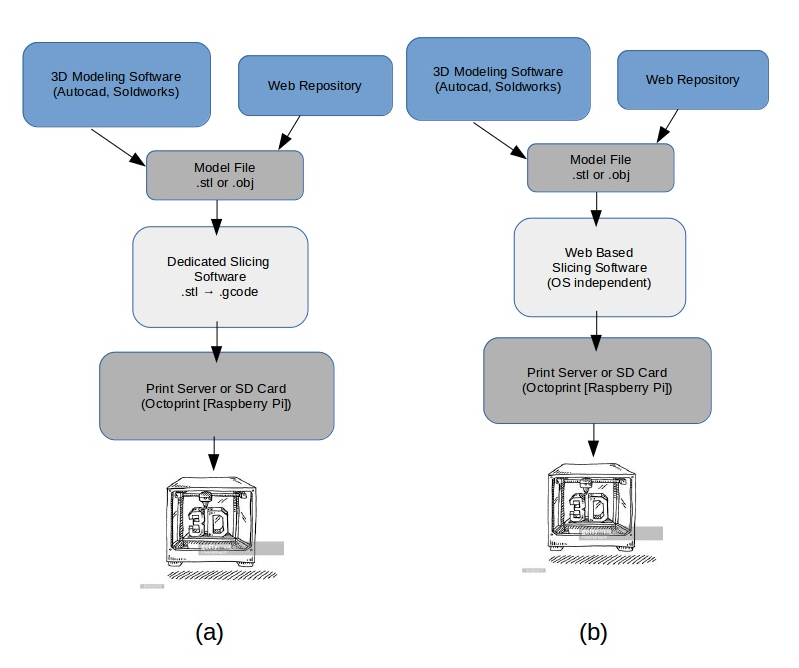
\includegraphics[width=\linewidth]{basic-process-3D-printing}
  \caption{(a) High level view of the normal 3D printing process. (b) High level view of proposed new process using WebSlicer.}
\end{figure}


\section{The RepRap Idea}
\paragraph{}
The Replication Rapid-Prototyper Project (RepRap) is a movement with the goal of providing Open-source, diy 3D printers at low cost.
RepRap printers are 3D printers with the additional ability to produce most of the parts necessary to assemble another identical printer.
This idea also extends outside of hardware but to the software as well.
Much of the software available for RepRap style printers are open source projects put together by the community.

\section{Sudden Growth Of 3D Printing}
\paragraph{}
In an article written by Forbes they did an analysis of the current market trend for 3D printing and were surprised to find that it is becoming one of the fastest growing emerging markets.
"According to Wohlers Report 2014, the worldwide 3D printing industry is now expected to grow from \$3.07 billion in revenue in 2013 to \$12.8 billion by 2018, and exceed \$21 billion in worldwide revenue by 2020". \citet{forbes3D}
One reason that 3D printing has been reaching more people is the availability of the RepRap designs.
Additionally, to build a 3D printer from a kit only requires basic hand tools and basic electronics skills which means that it has been opened up to a much broader audience.

\section{Purpose of This Research}
\paragraph{}
The purpose of this research is to construct a web based slicer and make it simple for a user, who knows hardly anything about 3D printing, to slice models and run their 3D printer.
This will make 3D printing much more approachable for occasional users who are not prepared to spend thousands of dollars on a professional machine and software.
Additionally, this opens up opportunities for educators in STEM programs to teach students about 3D printing in a simple and practical way.
Under normal circumstances this would not be a feasible project for a year long Masters thesis.
However, many of the technologies required to complete this project exist in varying states of completeness.
Putting them together will be the subject of this study.


\section{Research Objectives}
\paragraph{}
This research has several milestones which must be met for this thesis to be considered complete.
These milestones are in no particular order.
However, several of them must be completed before allowing other milestones to be completed as detailed below.

\subsection{Wrap CuraEngine}
\paragraph{}
CuraEngine is an open-source slicing engine designed to take model files in .stl file format and convert them into G-code for 3D printing.
For this project, wrapping this code and making it callable from the web is the heart of this application.

\subsection{Design intuitive web interface}
\paragraph{}
This project requires both an intuitive and easy to way to slice a model file for 3D printing.
This would be done using Bootstrap and AngularJS because they are both scalable and flexible for almost any web design.
These technologies also allow for small scale or even mobile use.

\subsection{Run beta testing with actual users}
\paragraph{}
No research would be complete without testing the software in question.
Running a closed beta test of this software is a milestone that must be met as one of the major aspects of this application is its usability.

\section{Existing Technology}
% Talk about Astroprint 2 and why its not the full solution.
\paragraph{}
%3.1 AstroPrint 2
AstroPrint is an all included cloud operating system for 3D printers.
It attempts to encompass the entire package of 3D printing to a dedicated Raspberry Pi, or similar computer system.
It is also one of the only software platforms that currently exists that attempts to do web based slicing.
Unfortunately, the AstroPrint software tries to accomplish too many tasks at once and has become somewhat like a Swiss army knife as it is capable of many tasks but can only do a few tasks well.
Additionally, their cloud based slicing software, while being reasonably fast, lacks any support for reviewing the sliced model.
This review stage is critical for anyone who is printing something that will take more than a few hours to complete.

\section{Thesis Map}
% This is where a design for reading this research should be shown so that someone can easily figure out what they want to read about.
% ideally this should be an ordered list similar to the index except more broad and with descriptions
\paragraph{}
\begin{itemize}
\item Chapter 2, Background and design choices.
\item Chapter 3, Software architecture review.
\item Chapter 4, Client side in detail. 
\item Chapter 5, Server side in detail.
\item Chapter 6, Discussion about usability testing and further improvements.
\end{itemize}

